\documentclass[12pt]{article}
\usepackage{geometry} 
\geometry{margin=1in}
\geometry{a4paper} 


\usepackage{textcomp}
\usepackage{booktabs}
\usepackage{array}
\usepackage{paralist}
\usepackage{verbatim} 
\usepackage{subfigure}
\usepackage{graphicx,caption}
\usepackage{placeins}
\usepackage{lipsum}
\usepackage{xcolor}
\usepackage{dcolumn}
\usepackage{sectsty}
\allsectionsfont{\sffamily\mdseries\upshape}
\usepackage{gensymb,amsmath,mathtools,amssymb}
\usepackage{flafter}
%\usepackage{parskip}
\usepackage[utf8]{inputenc}
\usepackage[english]{babel}
\usepackage{tocbibind}
\usepackage[toc,page]{appendix}
\captionsetup{width=\linewidth}
\usepackage{bm}
\usepackage{url}
\usepackage{empheq}

\newcommand{\half}{\frac{1}{2}}


\graphicspath{{./figs/}}


\title{Passive Flight Solution}
\author{Devansh Agrawal}
%\date{} 


\begin{document}

\maketitle


\section{Problem statement}

The dynamics of a rocket flying along the vertical axis (without thrust) can be written as

\begin{align}
\dot{h} &= v\\
\dot{v} &= -\frac{D}{m} - g = -\beta v^2  - g
\end{align}
where I have defined a modified ballistic coefficient
\begin{equation}
\beta = \frac{1}{2} \rho \frac{C_D A}{m}
\end{equation}

Since there is no thrusting, the mass is constant, and therefore $\beta$ is also constant. 

Further we assign the following boundary conditions, 

\begin{align}
h(0) &= h_0\\
v(0) &= v_0\\
v(t_f) &= 0
\end{align}

We wish to solve these equations, and determine the coasting distance. 


\section{Coasting Distance}

Using Mathematica's DSolve function, we can solve this non-linear coupled ode. Mathematica returns two solutions (which have been simplified here)\footnote{$\log$ here refers to the natural logarithm}:

Solution 1 (invalid):
\begin{align}
h(t) &=h_0 + \frac{\log \left(\cos \left(\sqrt{\beta  g}(t_f-t)\right)\right)}{\beta }-\frac{\log \left(-\sqrt{\frac{g}{g+\beta  v_0^2}}\right)}{\beta }\\
v(t) &=\sqrt{\frac{g}{\beta }} \tan \left(\sqrt{\beta  g}(t_f-t)\right)
\end{align}

and solution 2 (valid):
\begin{align}
h(t) &=h_0 + \frac{\log \left(\sqrt{1+\frac{\beta  v_0^2}{g}} \cos \left(\sqrt{\beta  g}(t_f-t)\right)\right)}{\beta } \label{eqn:h}\\
v(t) &= \sqrt{\frac{g}{\beta }} \tan \left(\sqrt{\beta  g}(t_f-t)\right) \label{eqn:v}
\end{align}

Notice, that due to the second logarithm in solution 1, it must be invalid\footnote{or if you think about expanding the log(negative square root()) into negative half log(), the expression turns out to be same as solution 2}, and that the velocity in both solutions are identical. Therefore, solution 2 is the accurate flight path. 

Immediately we can see from eqn~\ref{eqn:h} that the remaining height to go for the rocket is 
\begin{equation}
\boxed{\Delta h = h(t_f) - h_0 = \frac{1}{\beta} \log \left(\sqrt{1+\frac{\beta  v_0^2}{g}} \right)}
\end{equation}

In the limit that drag is insignificant $\beta \rightarrow 0$, and the equation correctly approaches the kinematic result, 

\begin{equation}
\lim_{\beta\rightarrow0} \Delta h = \frac{1}{2} \frac{v_0^2}{ g}
\end{equation}

The figure shows the results plotted. 


%\FloatBarrier
\begin{figure}[htbp]
   \centering
   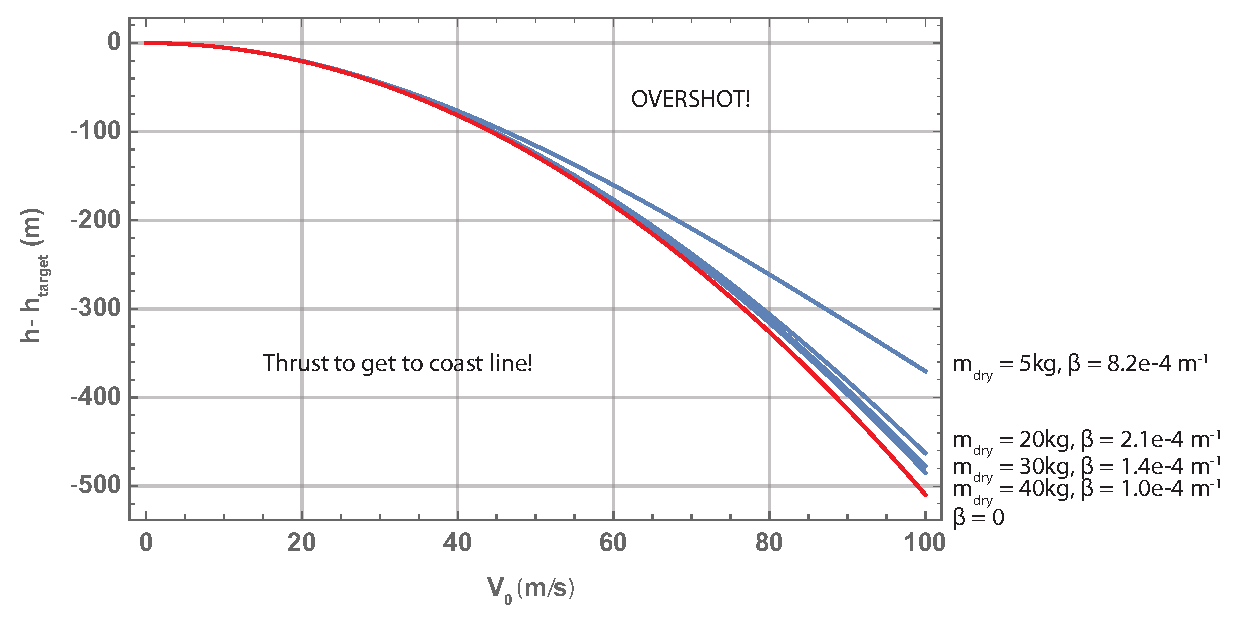
\includegraphics[width=0.8\linewidth]{coast_regions}
   \caption{This figure shows the combination of height to target and current flight speeds that will allow the rocket to coast to the target height. We see little dependence on the dry mass in the range of masses we are interested in. It is extremely important not to overshoot this line. The red lines shows the limiting case where the drag force can be neglected, and is a nice proxy for the case that drag cannot be accurately modelled.}
   \label{fig:}
\end{figure}
%FloatBarrier

%\FloatBarrier
\begin{figure}[htbp]
   \centering
   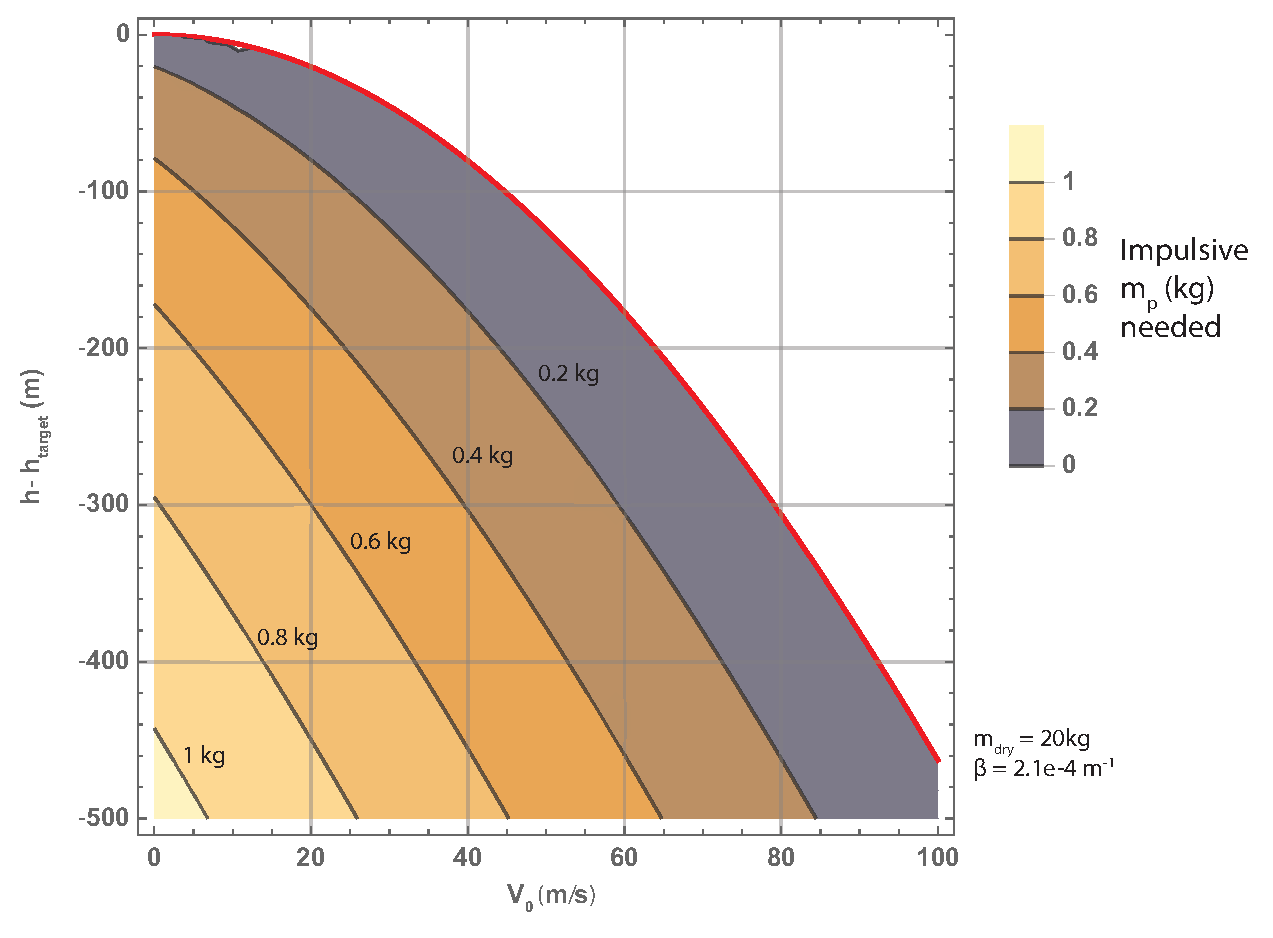
\includegraphics[width=0.8\linewidth]{impulsiveCorrection.eps}
   \caption{This figure shows the amount of propellant needed if an impulsive manoeuvre is to be used to get the current (h,v) point onto the coasting line (ie moving sideways on the graph). It is computed for a specific case of 20~kg dry mass, and shows that rather small amounts of propellant are needed (note, the propellant mass needed scales basically linearly with dry mass though). Less propellant should be needed for a non-impulsive manoeuvre. Therefore we could design the open loop trajectory aiming for 40~m/s at 300 m remaining, which gives us on the order 4 seconds to recompute and implement the final thrusting.}
   \label{fig:}
\end{figure}
\FloatBarrier


\section{Full Flight Path}

If we assume $v$ behaves well, we can solve eqn~\ref{eqn:v} for the final time using $t=0$,  and determine the flight profile:

\begin{empheq}[box = \fbox]{align}
t_f &= \frac{1}{\sqrt{\beta g}} \arctan{\left(v_0 \sqrt{\frac{\beta}{g}}\right)}\\
h(t) &= h_0 + \frac{1}{\beta} \log \left[\cos \left(t \sqrt{\beta  g}\right)+\sqrt{\frac{\beta  v_0^2 }{ g}} \sin \left(t \sqrt{\beta  g}\right)\right]\\
v(t) &= \sqrt{\frac{g}{\beta }} \tan \left[\arctan\left(v_0\sqrt{\frac{\beta }{g}}\right) - t \sqrt{\beta  g}\right]
\end{empheq}


While these expressions look complicated, they are in closed form, and therefore are extremely useful!

Note, these derivations ignore the change in drag coefficient with mach number, and the change in air density with altitude. 




%\bibliographystyle{unsrt}
%\bibliography{biblio}

\end{document}























